\PassOptionsToPackage{unicode}{hyperref}
\documentclass[aspectratio=1610, professionalfonts, 9pt]{beamer}

\usefonttheme[onlymath]{serif}
\usetheme[showtotalframes]{tudo}


\usepackage{polyglossia}
\setmainlanguage{english}

% Mathematik
\usepackage{mathtools}

% Enable Unicode-Math and follow the ISO-Standards for typesetting math
\usepackage[
  math-style=ISO,
  bold-style=ISO,
  sans-style=italic,
  nabla=upright,
  partial=upright,
]{unicode-math}
\setmathfont{Latin Modern Math}

% nice, small fracs for the text with \sfrac{}{}
\usepackage{xfrac}

\usepackage{multicol}
\usepackage{graphicx}
\usepackage{amssymb}
\usepackage{amsmath}
\usepackage{xparse}
\usepackage{braket}
\usepackage{units}
\usepackage[locale=DE,separate-uncertainty=true,per-mode=reciprocal,output-decimal-marker={,},]{siunitx}
\sisetup{
  round-mode          = places, % Rounds numbers
  round-precision     = 2, % to 2 places
}
\usepackage[section]{placeins}
\usepackage{pdflscape}
\usepackage{expl3}
\usepackage{bookmark}
\usepackage{booktabs}
%Komma als Dezimaltrenner in der mathe Umgebung, um in Umgebungen wie [0, 2] ein Leerzeichen nach dem Komma zu erhalten einfach eins setzen
\usepackage{icomma}
\usepackage{cancel}

\usepackage[
  backend=biber,   % use modern biber backend
  autolang=hyphen, % load hyphenation rules for if language of bibentry is not
                   % german, has to be loaded with \setotherlanguages
                   % in the references.bib use langid={en} for english sources
]{biblatex}
\addbibresource{references.bib}  % die Bibliographie einbinden
\DefineBibliographyStrings{german}{andothers = {{et\,al\adddot}}}



\usepackage{hyperref}
\usepackage{subfigure}
\usepackage[labelformat=empty]{caption}





%%%%%%%%%%%%%%%%%%%%%%%%%%%%%%%%%%%%%%%%%%%%%%%%%%%%%%%%%%%%%%%%%%%%%%%%%%%%%%%%
%%%%%-------------Hier Titel/Autor/Grafik/Lehrstuhl eintragen--------------%%%%%
%%%%%%%%%%%%%%%%%%%%%%%%%%%%%%%%%%%%%%%%%%%%%%%%%%%%%%%%%%%%%%%%%%%%%%%%%%%%%%%%

%Titel:
\title{Detektion von Fake News}
%Autor
\author{Lars Möllerherm und Clemens Vorsmann}
%Lehrstuhl/Fakultät
\institute{Fakultät Physik}

\AtBeginSection[]{
    \begin{frame}
      \vfill
      \centering
      \usebeamerfont{title}\insertsectionhead\par%
      \vfill
    \end{frame}
}

\begin{document}



  \begin{frame}
    \titlepage
  \end{frame}

  \begin{frame}
    \frametitle{Definition und Motivation}
    \begin{itemize}
      \item Motivation:
      \begin{itemize}
        \item Fake News wurde zum Anglizismus des Jahres 2016 gewählt\cite{angli}.
        \item Größer werdende Rolle in unserer Gesellschaft.
        \item Falsch-Informationen werden besser.
        \item Natürlicher "Bullshit"-Filter funktioniert nicht mehr.
      \end{itemize}
    \end{itemize}
    \begin{columns}
      \column{0.6\textwidth}
      \begin{itemize}
        \item Definition:
        \begin{itemize}
        \item Es existiert der BS-Detector von Daniel Sieradski\cite{BS}.
        \item Beinhaltet Liste fragwürdigen URL's. Artikel mit Links auf diese URL's, 
            werden als BS gekennzeichnet.
        \item Ist es möglich, anhand des Sprachmusters, diese Kategorisierung vorzunehmen?
        \item Möglche Fake News Erkennung ohne URL Blacklist
        \end{itemize}
      \end{itemize}
      \column{0.4\textwidth}
      \begin{figure}
          
\includegraphics[width=\textwidth]{pictures/trump-fake-news.jpg}
          \caption{https://www.skeptiker.ch/was-sind-fake-news/}
          \label{}
        \end{figure}
      \end{columns}
  \end{frame}

  \begin{frame}
    \frametitle{Beschreibung des Datensatzes}
    \begin{columns}
      \column{0.5\textwidth}
      \begin{figure}
          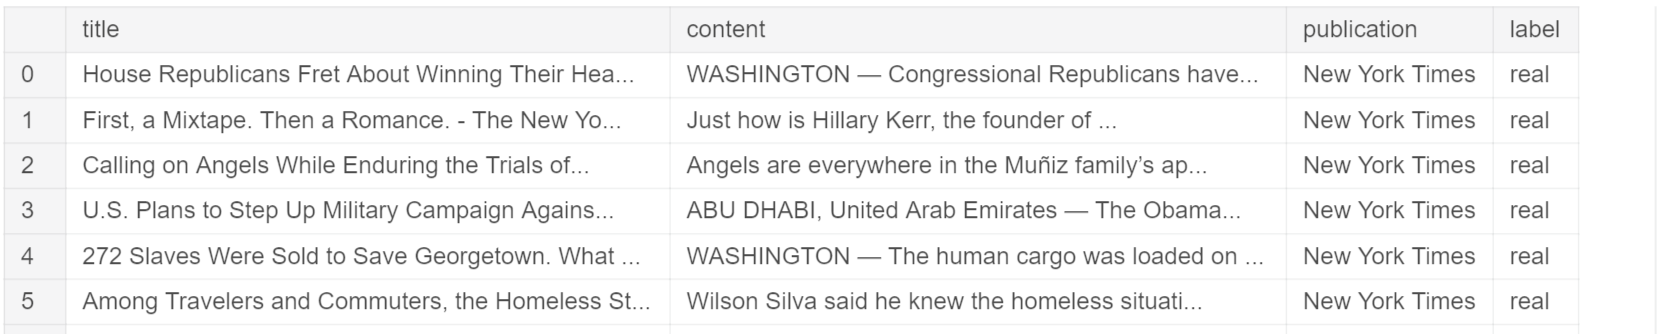
\includegraphics[width=\textwidth]{pictures/fake.PNG}
          \caption{https://www.skeptiker.ch/was-sind-fake-news/}
          \label{}
      \end{figure}
      \column{0.5\textwidth}
      \begin{itemize}
      \item 
      \end{itemize}
    \end{columns}
  \end{frame}

  \begin{frame}
    \frametitle{Mögliche Alternativ-Methode}
    \begin{figure}
          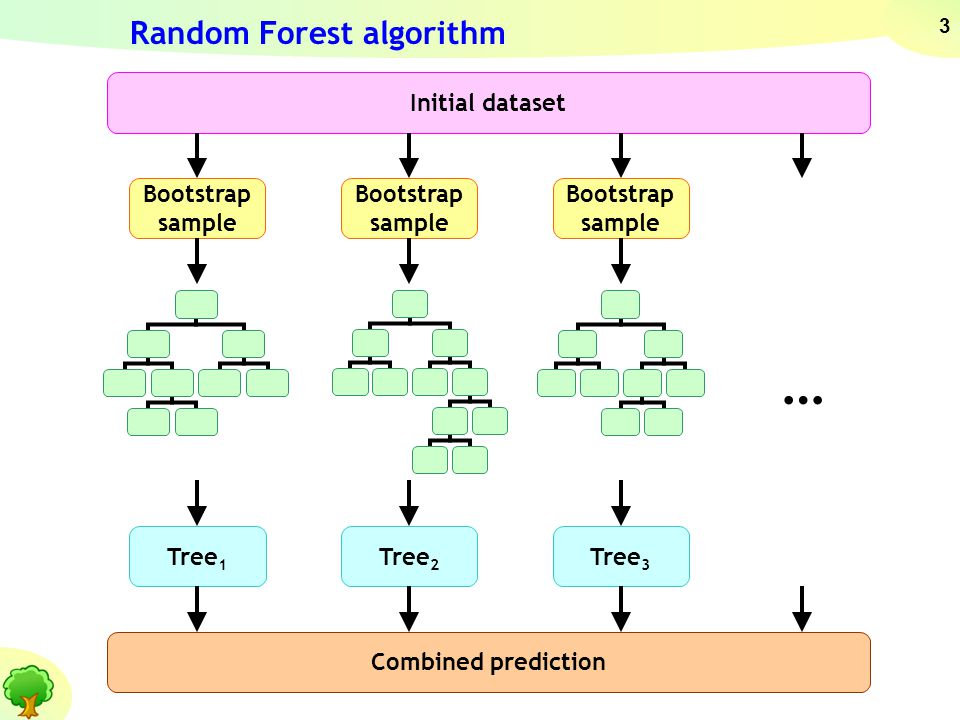
\includegraphics[width=\textwidth]{pictures/RF.jpg}
          \caption{Pavel Polishchuk}
          \label{}
      \end{figure}
  \end{frame}

\end{document}